%!TEX TS-program = pdflatex
%!TEX root = main.tex
%!TEX encoding = UTF-8 Unicode

\section{Implementation}
In this section I provide a high level description of the C++ implementation of an SDF Renderer utilizing sphere tracing.
The described code can be found at \href{https://github.com/Nyriu/RayTracer}{Nyriu/RayTracer}.

\subsection{Compiling}
The source code can be compiled with the common CMake workflow:
\begin{lstlisting}
mkdir build
cd build
cmake ..
make
cd ..
./main
\end{lstlisting}
The project was written and tested on a Manjaro operating system, but it should compile on other machines.
There are two major dependencies: SDL2 and OpenGL Mathematics (GLM).
The latter can be easily removed by re-implementing some of the matrix and vector operations.
SDL2 is used to open a window that shows the rendered images.
This dependence can be also removed by commenting out the relative lines from the \emph{Renderer} class and not compiling the \emph{Window} class.


\subsection{Classes and Structure}
The main header files and classes are:
\begin{itemize}
  \item \emph{ImplicitShape.h} in which is defined the homonymous abstract class and its children \emph{Sphere}, emph{Torus}, etc...
    Each class represents an implicit surface described via an SDF function, and provides methods to compute point-to-set distances and normal at a given point.
    The shapes have other properties such as the diffuse and specular colors.
    In this file are also defined the CSG operation, here considered as a particular case of implicit shape.
   Union, subtraction and intersection can be used to form a structure that resemble a binary tree;

  \item the \emph{Camera} is a perspective camera and can be placed in a scene, oriented with a target point or with a given view direction, and has a modifiable field of view;
  \item \emph{Ray} consists in a point and a direction and gives the possibility to calculate the ray position at a given $t$;

  \item \emph{Light.h} describes an abstract \emph{Light} class that is implemented with the \emph{PointLight} class.
    A light exposes publicly its color, position and intensity;

  \item a \emph{Scene} consists of a series of shapes, lights and a camera.
    The implementation offers methods to add and retrieve objects in the scene;

  \item the \emph{Tracer} implements the sphere tracing algorithm and is responsible of pixel shading.
    Here the ray's path is followed until its first bounce, then shadowing is verified and shading is computed.
    If there's no bounce then a default color is returned.

  \item the \emph{Renderer} asks the camera rays and passes them to the tracer.
    When the tracer has returned the pixel's color, the renderer saves it to an \emph{Image} that is then displayed in a \emph{Window} or saved to file;

  \item \emph{Color} abstraction of an RGB triplet;
  \item \emph{Image} squared 2D grid of pixels, each accessible and modifiable with $xy$ coordinates.
    As usual the top left corner is $(0,0)$, $x$ grows towards the right and $y$ towards the bottom;

  \item the \emph{Window} handles SDL calls to open, close and update an SDL window.

  \item \emph{geometry} contains geometric abstractions such as 3D points, vectors and matrices and operations on them;
  \item \emph{utilities.h} contains miscellaneous functions both used in the implementation and during implementation.
\end{itemize}
The file \emph{main.cpp} can be modified to load different scenes and to change the output image properties, here we can also enable or disable the SDL window rendering only to file in PPM format.
Inside \emph{scenes.cpp} different scenes are defined with different shapes and light as an example.
A scene should also contain a camera, if that's not the case the renderer's camera will be used (if provided).


\subsection{Limitations and Future Improvements}
The current implementation doesn't permit real time interaction.
That's because the code run exclusively on CPU and sequentially.
This limitation can be overcome re-implementing the shading part in parallel e.g. with CUDA.
Since each ray does not depend on the others, the ray computation can naturally benefit from parallelism.

As a consequence of the computation being sequential, the rendering has a single buffer.
Thus the frame rate is limited by the generation of every single image.
Also the code waits the image to be fully completed before showing it to the user.

Another limitation is that the scene must be described in C++ and there is no hot reloading if something in the scene changes.
In future could be interesting to create a simple parser for plain text files that describe scenes.

\clearpage
\subsection{Generated Images}

\begin{figure}[!htb]
  \centering
  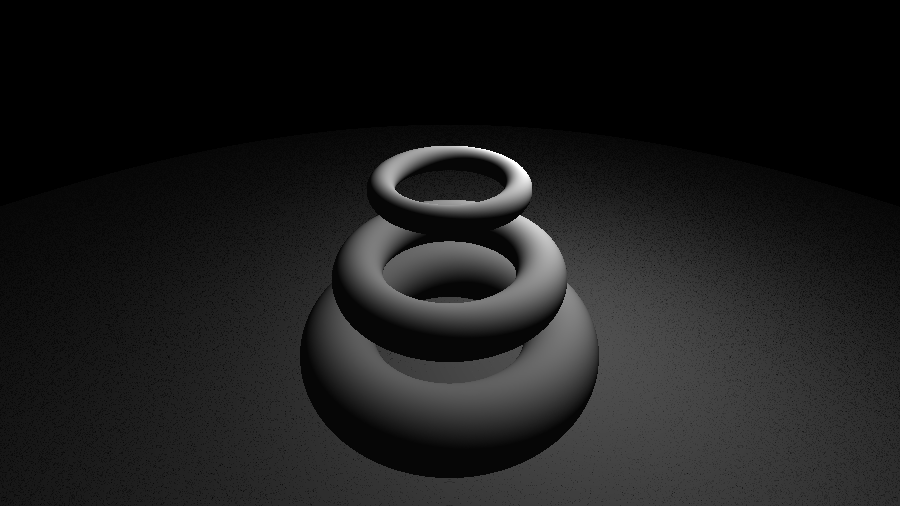
\includegraphics[width=\linewidth]{toruses_no_shadow.png}
  \caption{Three grey toruses, a white point light, a soft ambient light, and no shadowing.}
  \label{fig:toruses_no_shadow}
\end{figure}

\begin{figure}[!htb]
  \centering
  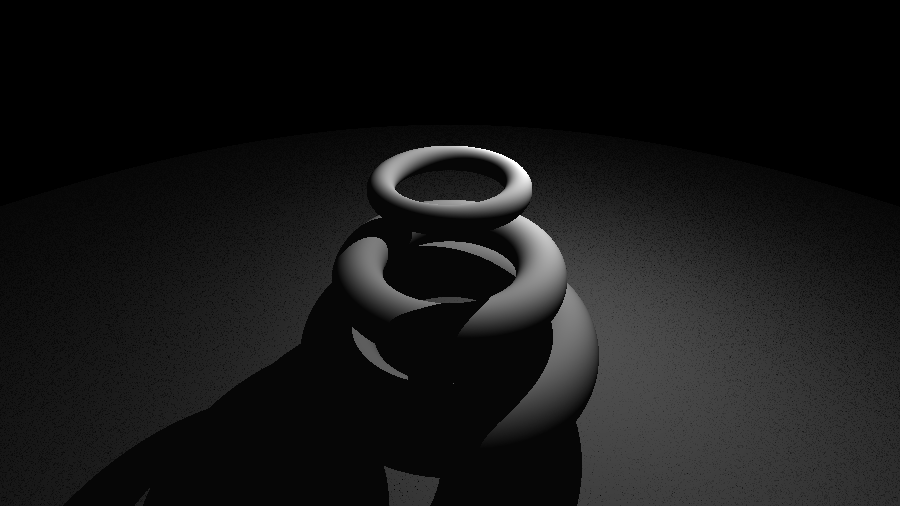
\includegraphics[width=\linewidth]{toruses_shadow.png}
  \caption{As \autoref{fig:toruses_no_shadow} but with shadowing enabled. Note how the image gains credibility.}
  \label{fig:toruses_shadow}
\end{figure}

\clearpage

\begin{figure}[!htb]
  \centering
  
\includegraphics[width=\linewidth]{subtraction.png}
  \caption{The result of a subtraction between the union of three grey toruses and a sphere.
    Note that the object cast (correctly) shadows on itself.
    The blue color is given by an ambient light.
  }
  \label{fig:subtraction_3D}
\end{figure}


\begin{figure}[!htb]
  \centering
  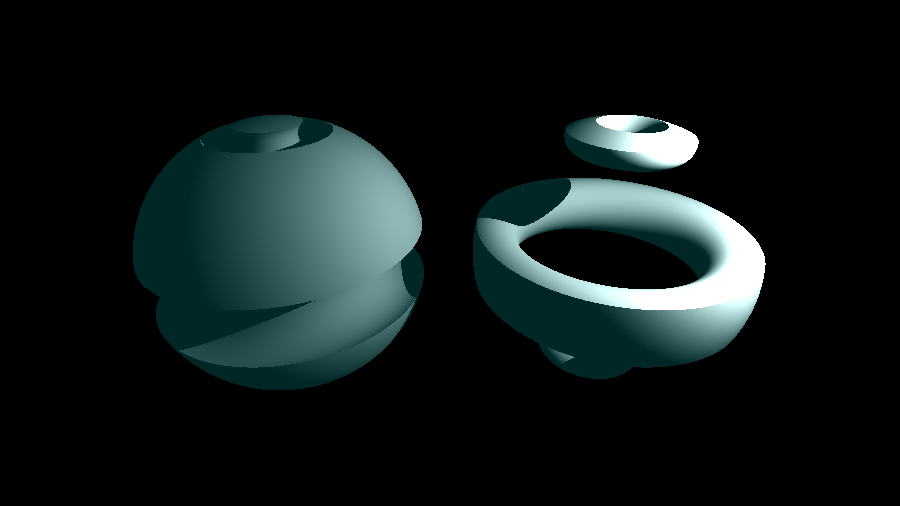
\includegraphics[width=\linewidth]{subtraction_intersection.png}
  \caption{
    Similar as \autoref{fig:subtraction_intersection} but now we subtract the (union of) toruses form the sphere.
    At the right the intersection of the sphere and the (union of) toruses.
    As before the color is given by an ambient light, because all shapes are grey.
    Note the correct self shadowing both on subsection and interaction.
  }
  \label{fig:subtraction_intersection}
\end{figure}

\clearpage
\begin{figure}[!htb]
  \centering
  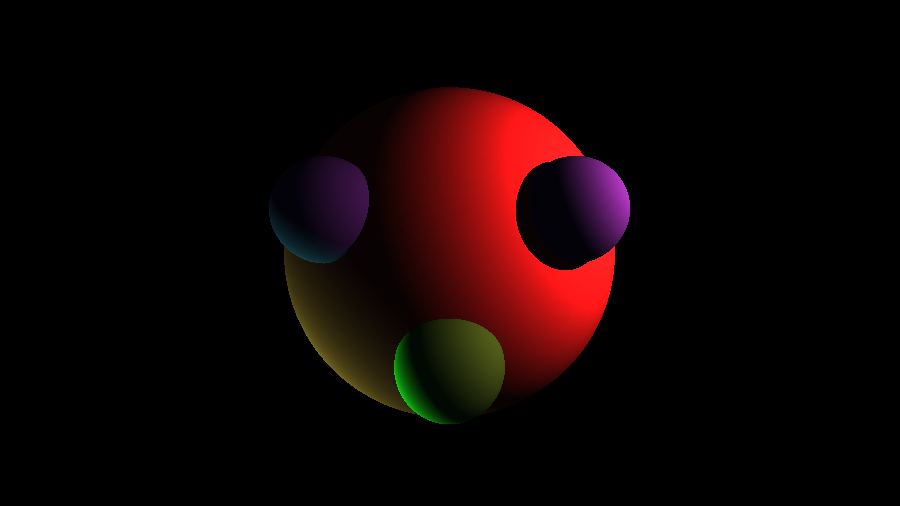
\includegraphics[width=\linewidth]{lights_and_diffuse.png}
  \caption{
    Four sphere with different colors lightened by two light of different colors.
    Note how the two sphere in the top left and right have the same color but the one to the left reflects different components of the left light.
  }
  \label{fig:lights_and_diffuse}
\end{figure}

One last note about self-hit of shadows rays.
When a shadow ray bounces if the first step is too small we risk to consider the analyzed point as in shadow because we didn't move the point far enough from the current surface.
This result in the point shadowing itself, giving the black pixels on the sphere surface of \autoref{fig:csg} at \autopageref{fig:csg} and on the toruses of \autoref{fig:toruses} at \autopageref{fig:toruses}.
Since we have to handle also CS shapes we can not simply exclude the current surface from the hittable ones.
Removing it will cause the shadows around the top right sphere in \autoref{fig:lights_and_diffuse} to disappear, but these shadows are correct.
The implemented solution is to move the origin of the shadow ray along the surface normal (at the considered point).
